\chapter{Wstęp}\label{chap:wstep}

\section{Kontekst problemu i znaczenie badań}\label{sec:kontekst-problemu}

Każdego roku do schronisk dla zwierząt na całym świecie trafiają miliony bezdomnych psów i kotów, co stanowi ogromne wyzwanie organizacyjne i logistyczne. W samych Stanach Zjednoczonych szacuje się, że rocznie do schronisk trafia około 6 milionów psów i kotów \cite{SAC2024,aspca2024}. Efektywne zarządzanie taką liczbą podopiecznych wymaga zapewnienia odpowiedniej opieki, zasobów i przestrzeni każdemu zwierzęciu, przy jednoczesnym dążeniu do jak najszybszego znalezienia mu nowego domu. Jednym z kluczowych wskaźników skuteczności pracy schroniska jest czas pobytu zwierzęcia pod jego opieką (ang. \emph{Length of Stay}, LOS). Im krótszy jest LOS, tym mniejsze obciążenie dla zwierzęcia (ograniczenie stresu, ryzyka chorób i zgonu) oraz dla placówki (niższe koszty utrzymania i więcej wolnego miejsca dla kolejnych potrzebujących).

Coraz więcej schronisk przyjmuje filozofię „\emph{No-Kill}”, która zakłada unikanie eutanazji zdrowych zwierząt poprzez osiąganie bardzo wysokiego odsetka adopcji i uratowań. Przykładem spektakularnego sukcesu podejścia \emph{No-Kill} jest \emph{Austin Animal Center} (AAC) w Teksasie. Od 2011~roku miasto Austin może poszczycić się mianem największego miasta w USA o statusie \emph{No-Kill}, utrzymując współczynnik uratowań (ang. \emph{live-release rate}) powyżej 90\% \cite{Austin2010}. Schronisko AAC przyjmuje ponad 18 tysięcy zwierząt rocznie \cite{Austin2010}, co czyni je jedną z największych tego typu placówek komunalnych w kraju i jednocześnie stawia przed nim ogromne wymagania w zakresie efektywnego wykorzystania danych i zasobów. Dążenie do utrzymania wysokiego odsetka adopcji przy tak dużej skali działalności wymaga ciągłego usprawniania procesów i podejmowania trafnych decyzji operacyjnych.

W ostatnich latach zauważalny jest istotny zwrot od podejmowania decyzji w oparciu o doświadczenie i intuicję personelu ku podejściu opartemu na danych (\emph{data-driven}). Większość dużych schronisk gromadzi szczegółowe informacje o każdym przyjęciu i opuszczeniu zwierzęcia (intake \& outcome), jednak w wielu przypadkach dane te nie są w żadnym stopniu wykorzystywane do wyciągania praktycznych wniosków. Zastosowanie nowoczesnych metod analizy danych i uczenia maszynowego otwiera możliwość lepszego zrozumienia, jakie czynniki sprzyjają szybkim adopcjom, a jakie wiążą się z dłuższym pobytem zwierząt w schronisku lub -- w skrajnych przypadkach -- ich uśpieniem. Modele predykcyjne mogą pomóc przewidywać prawdopodobieństwo adopcji konkretnego zwierzęcia oraz zidentyfikować obszary wymagające interwencji (np. grupy zwierząt o podwyższonym ryzyku długotrwałego pobytu). Tym samym, badania łączące dane schronisk z metodami \emph{machine learning} mają istotne znaczenie praktyczne: mogą przyczynić się do optymalizacji pracy schronisk, lepszego alokowania zasobów oraz, co najważniejsze, ratowania większej liczby zwierząt poprzez skracanie czasu oczekiwania na nowy dom i uniknięcie śmierci.

Analizowany w niniejszej pracy zbiór danych obejmuje 162\,390 dopasowanych epizodów pobytu (przyjęcie--wynik) zarejestrowanych w systemie AAC w latach 2013--2025, w tym 93\,805 epizodów dotyczących psów oraz 68\,585 dotyczących kotów.

\begin{figure}[htbp]
  \centering
  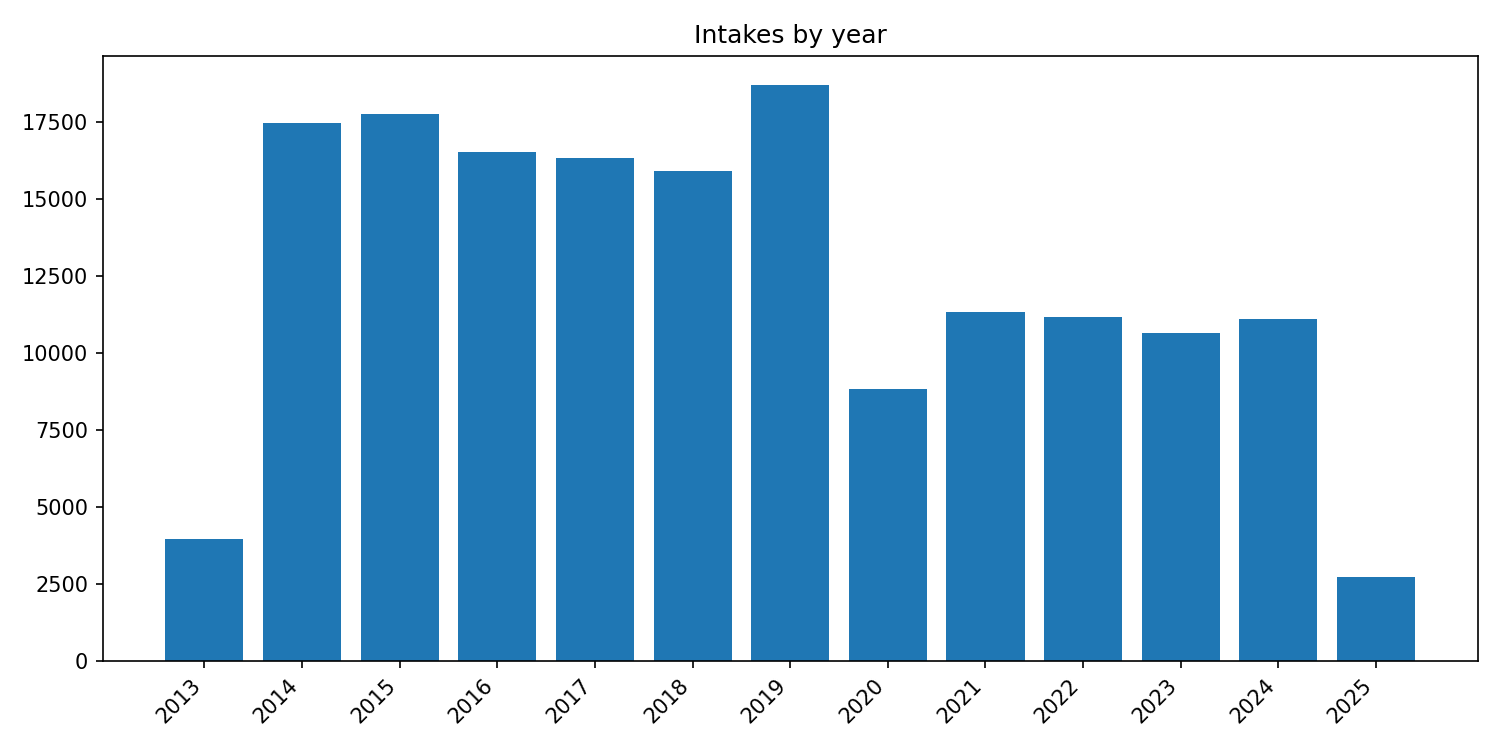
\includegraphics[width=0.88\textwidth]{../reports/figures/intakes_by_year.png}
  \caption{Liczba przyjęć zwierząt do schroniska Austin Animal Center w kolejnych latach (2013--2025). Wyraźnie widoczny jest spadek wolumenu przyjęć w latach 2020--2021 związany z ograniczeniami pandemii COVID-19, a następnie stopniowy powrót do wartości sprzed pandemii.}
  \label{fig:intakes_by_year}
\end{figure}

\begin{figure}[htbp]
  \centering
  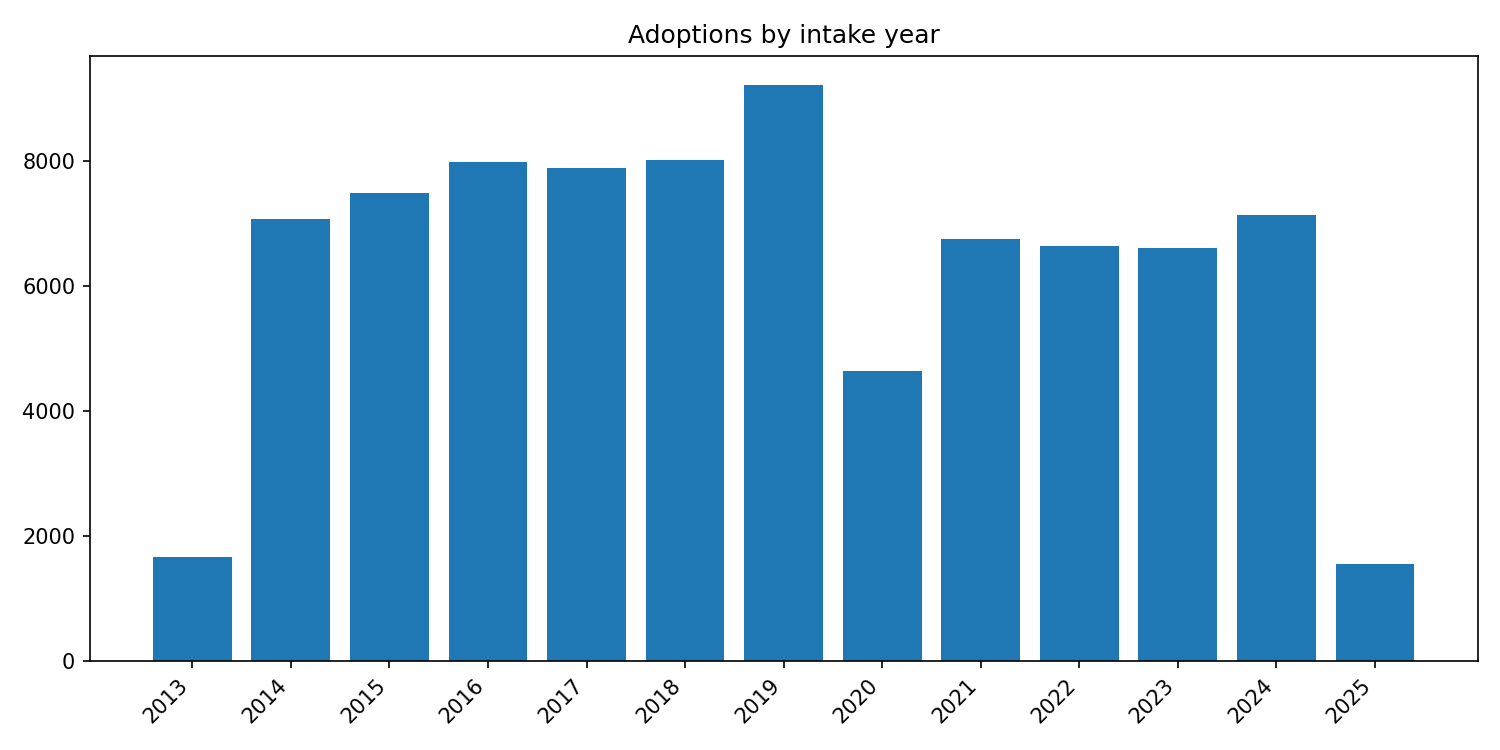
\includegraphics[width=0.88\textwidth]{../reports/figures/adoptions_by_year.png}
  \caption{Liczba adopcji zarejestrowanych w AAC w kolejnych latach (2013--2025). Zestawienie z Rysunkiem~\ref{fig:intakes_by_year} ilustruje zmienną relację między wolumenem przyjęć a skutecznością adopcji w poszczególnych latach.}
  \label{fig:adoptions_by_year}
\end{figure}

Dotychczasowe badania wykazały obiecujące rezultaty w zakresie predykcji adopcji z wykorzystaniem uczenia maszynowego. Bradley i Rajendran~\cite{Bradley2021} zaproponowali dwufazowy model predykcji czasu pobytu w schronisku, natomiast Sazara i Gao~\cite{Sazara2022} zastosowali algorytm CatBoost do przewidywania czasu adopcji, uzyskując wysoką trafność i identyfikując wiek oraz rasę jako najważniejsze cechy. Niniejsza praca rozszerza te podejścia o chronologiczny podział danych, analizę interpretowalności SHAP oraz wdrożenie interaktywnego systemu decyzyjnego.

Warto też wspomnieć o wymiarze etycznym. Dane wykorzystywane w niniejszej pracy pochodzą z publicznie dostępnych rejestrów Austin Animal Center i nie zawierają danych osobowych adopcjobiorców. Jednakże zastosowanie modeli predykcyjnych w kontekście schroniskowym wiąże się z ryzykiem utrwalenia istniejących uprzedzeń (np. dyskryminacji rasowej zwierząt). Dlatego model zaprojektowano jako narzędzie wspierające, a nie zastępujące, decyzje personelu schroniska.

\section{Cel, hipotezy i pytania badawcze}\label{sec:cel-hipotezy}

Celem niniejszej pracy jest opracowanie kompleksowego, zaawansowanego systemu analitycznego wykorzystującego metody uczenia maszynowego do prognozowania adopcji zwierząt na podstawie danych historycznych ze schroniska oraz identyfikacji najważniejszych czynników wpływających na przebieg tych adopcji. W szczególności praca skupia się na oszacowaniu prawdopodobieństwa adopcji oraz czasu oczekiwania na adopcję dla psów i kotów przyjętych do \emph{Austin Animal Center} w latach 2013–2025. Osiągnięcie celu naukowego wymaga zbudowania dokładnego modelu predykcyjnego, ale wyzwaniem może być również zadbanie o jego interpretowalność oraz użyteczność praktyczną dla nietechnicznych użytkowników.   Dlatego też celem wdrożeniowym jest implementacja systemu, który integruje powstały model w formie interaktywnej aplikacji (\emph{dashboard}) przeznaczonej dla personelu i wolontariuszy schroniska. System ten ma umożliwiać eksplorację wyników predykcji (np. przewidywanego czasu adopcji danego zwierzęcia) oraz przeprowadzanie analiz typu „co-jeśli” w celu wsparcia decyzji dotyczących działań ukierunkowanych na zwierzęta o obniżonych szansach adopcyjnych.

Równolegle, celem analitycznym niniejszej pracy jest pogłębiona identyfikacja tych cech zwierząt oraz czynników zewnętrznych, które istotnie wpływają na zmniejszenie prawdopodobieństwa adopcji, co może stanowić podstawę do dalszych interwencji, zmian w działaniach operacyjnych lub kampanii adopcyjnych ukierunkowanych na najbardziej narażone grupy.

Aby zrealizować powyższe cele, sformułowano następujące kluczowe pytania badawcze:

\begin{enumerate}\itemsep2pt
\item \label{rq:1} \textbf{Które zmienne opisujące zwierzę oraz okoliczności jego przyjęcia do schroniska najsilniej wpływają na prawdopodobieństwo szybkiej adopcji?} Jakie cechy (np. wiek, rasa, umaszczenie, płeć, stan zdrowia, typ przyjęcia) wykazują największą moc predykcyjną w kontekście skrócenia lub wydłużenia czasu pobytu zwierzęcia w schronisku?
\item \label{rq:2} \textbf{Jak złożone modele uczenia maszynowego wypadają na tle prostszych metod w zadaniu przewidywania adopcji zwierząt?} Innymi słowy, czy zastosowanie algorytmów klasy \emph{ensemble} (np. gradient boosting w modelach XGBoost/CatBoost) zapewnia wyraźnie lepszą trafność prognoz niż podstawowe podejścia bazowe (takie jak proste modele regresyjne lub losowe strategie decyzji)?
\item \label{rq:3} \textbf{Czy istnieją istotne różnice w wzorcach adopcji między psami a kotami oraz jak te wzorce zmieniały się w czasie?} Pytanie to dotyczy zarówno ewentualnych odmiennych czynników wpływających na adopcje w zależności od gatunku, jak i trendów czasowych (np. czy w kolejnych latach obserwuje się poprawę skuteczności adopcji, zmiany sezonowe itp.).
\end{enumerate}

Mając na uwadze powyższe pytania oraz przegląd literatury przedmiotu, przyjęto również kilka hipotez badawczych, które zostaną zweryfikowane w toku analizy:

\begin{description}\itemsep2pt
\item[H1:] Sposób, w jaki zwierzę trafia do schroniska (np. jako bezdomna znajda przywieziona przez służby miejskie, czy jako zwierzę oddane bezpośrednio przez właściciela), ma istotniejszy wpływ na prawdopodobieństwo i tempo jego adopcji niż cechy wyglądu. Innymi słowy, zakłada się, że typ przyjęcia (ang. \emph{intake type}) stanowi silniejszy prognostyk sukcesu adopcyjnego niż przynależność do konkretnej rasy.

\item[H2:] Występuje wyraźny efekt sezonowości w przebiegu adopcji. Pewne okresy w roku (np. miesiące letnie lub okolice przerw świątecznych) sprzyjają szybszym adopcjom, skracając średni czas pobytu zwierząt w schronisku, podczas gdy w innych okresach tempo adopcji spada. Hipoteza ta opiera się na założeniu, że czynniki zewnętrzne (takie jak wakacje, kampanie społeczne czy warunki pogodowe) wpływają na popyt na adopcje.

\item[H3:] Wiek zwierzęcia ma istotny wpływ na jego szanse adopcyjne – młodsze zwierzęta są adoptowane szybciej niż starsze. Zgodnie z obserwacjami z praktyki schroniskowej, szczenięta i kocięta cieszą się większym zainteresowaniem niż osobniki dorosłe lub starsze.

\item[H4:] Umaszczenie zwierzęcia wpływa na prawdopodobieństwo adopcji – zwierzęta o ciemnym umaszczeniu (np. czarne psy i koty) są adoptowane rzadziej. Zjawisko to, znane jako \emph{black dog syndrome}, jest często przytaczane w mediach, choć literatura naukowa nie jest w tej kwestii jednogłośna \cite{svoboda2015}. W ramach pracy zweryfikowane zostanie, czy w danych z AAC zjawisko to jest rzeczywiście obserwowalne.


\item[H5:] Pandemia COVID-19 (2020--2021) spowodowała istotne zmiany w dynamice adopcji zwierząt: w roku 2020 odnotowano wzrost wskaźnika adopcji i skrócenie mediany czasu pobytu (tzw.\ \emph{pandemic adoption surge}), natomiast rok 2021 przyniósł częściowe odwrócenie tego trendu wraz ze stopniowym powrotem do normalnej działalności schroniska.
\end{description}


Powyższe hipotezy zostaną poddane weryfikacji w dalszych rozdziałach pracy. Analiza ich trafności pozwoli nie tylko odpowiedzieć na postawione pytania badawcze, lecz także lepiej zrozumieć dynamikę procesów adopcyjnych. Praca obejmuje pełny cykl projektowy: od analizy danych i budowy modeli predykcyjnych po wdrożenie działającego systemu wspierającego decyzje w schronisku.

\begin{table}[htbp]
\centering
\caption{Zestawienie głównych hipotez badawczych weryfikowanych w pracy.}
\label{tab:hipotezy_podsumowanie}
\renewcommand{\arraystretch}{1.3}
\begin{tabular}{|c|p{12cm}|}
\hline
\textbf{Identyfikator} & \textbf{Treść hipotezy} \\
\hline
H1 & Typ przyjęcia do schroniska ma istotniejszy wpływ na prawdopodobieństwo i tempo adopcji niż cechy wyglądu (np. rasa). \\
\hline
H2 & Występuje wyraźna sezonowość w adopcjach, wpływająca na czas pobytu zwierząt w schronisku w zależności od pory roku. \\
\hline
H3 & Młodsze zwierzęta (szczenięta, kocięta) mają wyższe szanse na szybką adopcję w porównaniu do starszych osobników. \\
\hline
H4 & Zjawisko ,,black dog syndrome'' (rzadsze adopcje zwierząt o ciemnym umaszczeniu) jest zauważalne w analizowanym zbiorze danych. \\
\hline
H5 & Pandemia COVID-19 (2020--2021) wpłynęła na dynamikę adopcji oraz zmiany w średnim czasie pobytu zwierząt. \\
\hline
\end{tabular}
\end{table}

\section{Zakres i struktura pracy}\label{sec:zakres-struktura}

Zakres analizy obejmuje dane historyczne pochodzące z \emph{Austin Animal Center} z lat 2013–2025, które zawierają informacje zarówno o przyjęciach zwierząt do schroniska (\emph{intake}), jak i o ich dalszych losach (\emph{outcome}, w szczególności adopcjach). Dane te pozwalają prześledzić pełny cykl pobytu zwierzęcia w schronisku – od momentu znalezienia lub oddania, aż do chwili adopcji bądź innego zakończenia opieki. W pracy skoncentrowano się na dwóch dominujących w schronisku gatunkach, tj. psach i kotach, z pominięciem mniej licznych gatunków egzotycznych. Analizy zostały przeprowadzone oddzielnie dla psów i kotów wszędzie tam, gdzie było to zasadne, aby uchwycić ewentualne różnice między tymi grupami. Pod względem merytorycznym praca łączy zagadnienia z obszaru nauk o danych (data science), uczenia maszynowego oraz inżynierii oprogramowania, co znajduje odzwierciedlenie w strukturze pracy.

\begin{figure}[htbp]
\centering
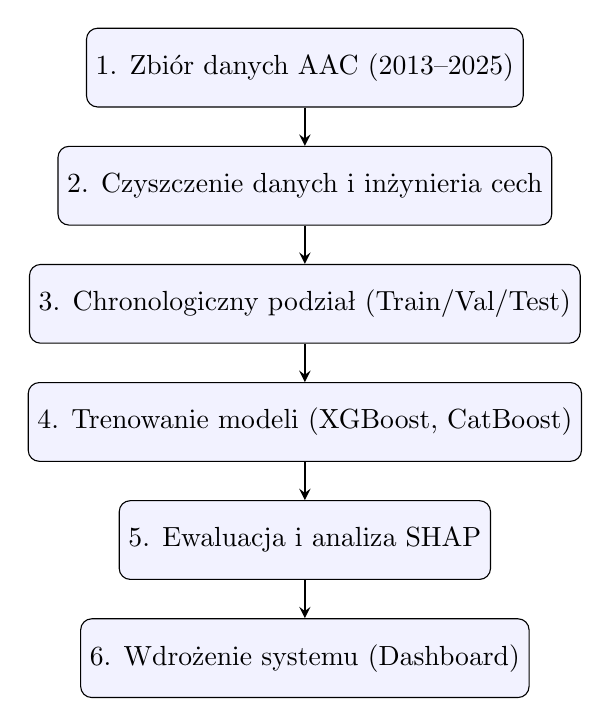
\begin{tikzpicture}[
    box/.style={rectangle, draw, rounded corners, minimum width=4cm, minimum height=1cm, align=center, fill=blue!5},
    arrow/.style={->, >=stealth, thick}
]
    \node[box] (data) at (0,0) {1. Zbiór danych AAC (2013--2025)};
    \node[box] (prep) at (0,-1.5) {2. Czyszczenie danych i inżynieria cech};
    \node[box] (split) at (0,-3) {3. Chronologiczny podział (Train/Val/Test)};
    \node[box] (model) at (0,-4.5) {4. Trenowanie modeli (XGBoost, CatBoost)};
    \node[box] (eval) at (0,-6) {5. Ewaluacja i analiza SHAP};
    \node[box] (deploy) at (0,-7.5) {6. Wdrożenie systemu (Dashboard)};

    \draw[arrow] (data) -- (prep);
    \draw[arrow] (prep) -- (split);
    \draw[arrow] (split) -- (model);
    \draw[arrow] (model) -- (eval);
    \draw[arrow] (eval) -- (deploy);
\end{tikzpicture}
\caption{Schemat blokowy metodyki badawczej i przepływu pracy (pipeline MLOps).}
\label{fig:ml_workflow}
\end{figure}

Rozdziały niniejszej pracy zostały ułożone w taki sposób, aby stopniowo wprowadzać czytelnika w temat i następnie przejść do szczegółów implementacyjnych rozwiązania. Rozdział 2 przedstawia przegląd literatury oraz teoretyczne podstawy związane z problematyką bezdomności zwierząt i adopcji w kontekście zarządzania schroniskami. Omówiono w nim kluczowe pojęcia (takie jak zasada \emph{No-Kill} czy metryki w pracy schronisk), a także metody analizy danych i algorytmy uczenia maszynowego wykorzystywane dotychczas do rozwiązywania podobnych problemów. Rozdział 3 zawiera opis danych wykorzystanych w badaniu – źródła i charakterystykę zbioru danych z AAC, sposób ich wstępnego przetworzenia oraz analizę eksploracyjną (EDA). Celem tej części jest zrozumienie struktury danych, wstępna identyfikacja trendów i potencjalnych zależności (np. typowe przedziały wiekowe zwierząt, sezonowość przyjęć i adopcji, itp.) oraz przygotowanie odpowiedniego zestawu cech do modelowania.

W Rozdziale 4 przedstawiono metodologię budowy modeli predykcyjnych. Opisano proces doboru cech (\emph{feature engineering}) istotnych z punktu widzenia przewidywania adopcji, a także wybrane algorytmy uczenia maszynowego. Szczególną uwagę poświęcono modelom typu \emph{gradient boosting}, takim jak XGBoost i CatBoost, ze względu na ich wysoką skuteczność w zadaniach z danymi tabelarycznymi. Omówiono też konfigurację tych modeli, strategie walidacji krzyżowej oraz metryki oceny, które posłużą do porównania ich z prostszymi modelami bazowymi. Rozdział 5 prezentuje uzyskane wyniki eksperymentów. Przedstawiono w nim porównanie jakości predykcji różnych modeli (m.in. porównanie modeli gradient boosting z modelami liniowymi) oraz analizę interpretowalności najlepszego modelu. Wykorzystano do tego techniki objaśniania decyzji czarnej skrzynki, w szczególności wartości SHAP (\emph{Shapley Additive Explanations}), które pozwalają określić wpływ poszczególnych cech (np. wieku, rasy, typu intaku) na przewidywane prawdopodobieństwo adopcji. Taka analiza dostarcza cennych informacji, czy model podejmuje decyzje w sposób zgodny z intuicją i wiedzą dziedzinową (np. czy potwierdza, że młode zwierzęta adoptowane są szybciej), a także może ujawnić nieoczywiste zależności w danych.

Rozdział 6 koncentruje się na aspekcie inżynierskim rozwiązania, opisując zastosowane podejście \emph{MLOps} do zapewnienia powtarzalności i niezawodności procesu analitycznego. W rozdziale tym omówiono, w jaki sposób stworzony model i towarzyszący mu kod zostały zintegrowane w ramach tzw. potoku przetwarzania (\emph{pipeline}) obejmującego: wersjonowanie danych i eksperymentów z użyciem narzędzia DVC (\emph{Data Version Control}), konteneryzację środowiska i zależności za pomocą Dockera, oraz automatyzację trenowania i wdrażania modelu z wykorzystaniem ciągłej integracji i dostarczania (CI/CD, np. na platformie GitHub Actions). Rozdział 7 przedstawia zaprojektowaną aplikację internetową (dashboard) służącą jako interfejs użytkownika dla opracowanego modelu. Opisano funkcjonalności prototypowej aplikacji stworzonej w technologii \emph{Streamlit} – m.in. możliwość sprawdzania prognoz dla wybranego zwierzęcia, symulacji scenariuszy (np. jak zmiana pewnych cech wpływa na przewidywane szanse adopcji), czy przegląd globalnych statystyk i trendów. Rozdział ten ukazuje, jak wyniki zaawansowanej analizy danych mogą zostać opakowane w przystępne narzędzie wspierające codzienną pracę schroniska. Wreszcie, Rozdział 8 to podsumowanie uzyskanych wyników oraz wnioski. Zawarto w nim omówienie stopnia realizacji celu pracy, weryfikację hipotez w świetle przeprowadzonych analiz oraz rekomendacje dotyczące wdrożenia wypracowanych rozwiązań w praktyce. Przedstawiono także propozycje dalszych kierunków rozwoju – zarówno jeśli chodzi o ulepszenia modelu (np. uwzględnienie dodatkowych danych lub zastosowanie alternatywnych technik uczenia), jak i rozszerzenie funkcjonalności systemu dla schroniska.

Niniejsza praca stanowi zatem połączenie badań nad danymi schroniska z praktycznym wdrożeniem rozwiązania informatycznego. Wkład własny autora przejawia się zarówno w warstwie analitycznej, jak i inżynierskiej. Od strony analitycznej obejmuje on przygotowanie i oczyszczenie zbioru danych, przeprowadzenie eksploracji w celu sformułowania hipotez, a następnie zaprojektowanie i wytrenowanie modeli predykcyjnych dostosowanych do specyfiki danych AAC. Od strony inżynierskiej, istotnym elementem pracy jest zaprojektowanie i zaimplementowanie kompletnego procesu MLOps. Obejmuje to m.in.: zautomatyzowanie procesu trenowania modelu i aktualizacji prognoz, wprowadzenie kontroli wersji dla danych i modeli (co zapewnia odtwarzalność wyników), konteneryzację aplikacji dla ułatwienia jej uruchomienia na dowolnej platformie, oraz integrację tych komponentów w ramach ciągłej integracji/dostarczania. Dodatkowo, autor stworzył aplikację webową, która udostępnia wyniki modeli szerszemu gronu odbiorców w intuicyjnej formie. Dzięki temu podejściu, praca nie tylko odpowiada na postawione pytania badawcze, ale również dostarcza narzędzia mogącego znaleźć praktyczne zastosowanie w poprawie efektywności działania schronisk dla zwierząt.
